	\documentclass[12]{article}%indispensable

%-----début préambule-----

\title{\LARGE\textbf{Les indispensables en mathématiques}}
\author{Loris Caruhel}
\date{22/03/2025}

% Packages utiles pour les maths
\usepackage{mathtools, amsmath, amssymb, amsthm}  % Symboles et environnements mathématiques
\usepackage[french]{babel} % Langue
\usepackage[utf8]{inputenc} % Encodage
\usepackage[T1]{fontenc} % Encodage
\usepackage{hyperref} % Pour les liens hypertexts
\usepackage{xcolor} % Couleur
\usepackage[a4paper, margin=1in]{geometry} % Ajuste les marges à 1 pouce
\usepackage{longtable}
\usepackage{graphicx} % Ajouter des images
\usepackage{float}
\usepackage{enumitem}
\usepackage{amsmath} % Pour les symboles mathématiques avancés
\usepackage{amsfonts} % Pour les polices de mathématiques
\usepackage{amssymb}  % Pour les symboles supplémentaires

% Les macros
\newcommand{\R}{\mathbb R}
\newcommand{\N}{\mathbb N}
\newcommand{\Z}{\mathbb Z}


\renewcommand{\arraystretch}{2} % Hauteur des cellules des tableaux

\setlength{\tabcolsep}{15pt} % Largeur des cellules
\setlength{\parindent}{0pt}

\setlist[itemize]{topsep=10pt, itemsep=10pt} % Ajuste les espacements des listes

% Environnement
\theoremstyle{plain}
\newtheorem{thrm}{Théorème}

\theoremstyle{definition}
\newtheorem{deff}{Définition}

\theoremstyle{remark}
\newtheorem{ex}{Exemple}
\newtheorem{rem}{Remarque}

%-----fin préambule-----

\begin{document}

\maketitle
\newpage

\large
\tableofcontents
\newpage

\section{Les fractions}
\large
\begin{itemize}
	\item \textbf{Addition :} \( \boxed{\dfrac{a}{b} + \dfrac{c}{d} = \dfrac{a \times d + b \times c}{b \times d}} \)
	\item \textbf{Soustraction :} \( \dfrac{a}{b} - \dfrac{c}{d} = \dfrac{a \times d - b \times c}{b \times d} \)
	\item \textbf{Multiplication :} \( \dfrac{a}{b} \times \dfrac{c}{d} = \dfrac{a \times c}{b \times d} \)
	\item \textbf{Division :} \( \dfrac{a}{b} \div \dfrac{c}{d} = \dfrac{a}{b} \times \dfrac{d}{c} = \dfrac{a \times d}{b \times c} \)
	\item \textbf{Simplification :} \( \dfrac{a \times k}{b \times k} = \dfrac{a}{b}, \quad k \neq 0 \)
	\item \textbf{Puissance :} \( \left (\dfrac{a}{b}\right )^{n} = \dfrac{a^{n}}{b^{n}} \)
	\item \textbf{Inverse :} \( \dfrac{1}{a} = a^{-1} \)
\end{itemize}
\newpage

\section{Les puissances}
\large
\begin{itemize}
	\item \textbf{Produit :} \( \boxed{a^{n}\times a^{m} = a^{n+m}} \)
	\item \textbf{Inverse :} \( \boxed{\frac{1}{a^{n}} = a^{-n}} \)
	\item \textbf{Quotient :} \( \boxed{\frac{a^{n}}{a^{m}} = a^{n-m}} \)
	\item \textbf{Puissance d'un quotient :} \( \boxed{\left( \frac{a}{b} \right)^n = \frac{a^n}{b^n}} \)
	\item \textbf{Puissance de puissance :} \( \boxed{(a^{n})^{m}=a^{n\times m}} \)
	\item \textbf{Exposants identiques :} \( \boxed{a^{n} \times b^{n} = (ab)^{n}} \)
	\item \textbf{Exposant fractionnaire :} \( \boxed{a^{\frac{m}{n}} = \sqrt[n]{a^m}} \)
	\item Pour $n$ \textbf{impair} \( \boxed{(-a)^{n} = -a^{n}} \)
	\item Pour $n$ \textbf{pair} \( \boxed{(-a)^{n} = a^{n}} \)
	\item \( \boxed{a^{0} = 1} \)
\end{itemize}
\newpage

\section{Les identités remarquables}
\large
\subsection{Puissance 2 :}
\begin{itemize}
	\item \(\boxed{(a + b)^2 = a^2 + 2ab + b^2} \)
	\item \(\boxed{(a - b)^2 = a^2 - 2ab + b^2} \)
	\item \(\boxed{(a + b)(a - b) = a^2 - b^2} \)
	\item \(\boxed{a^2 + b^2 = (a + b)^2 - 2ab}\)
\end{itemize}

\subsection{Puissance 3 :}
\begin{itemize}
	\item \(\boxed{(a + b)^3 = a^3 + 3a^2b + 3ab^2 + b^3}\)
	\item \(\boxed{(a - b)^3 = a^3 - 3a^2b + 3ab^2 - b^3}\)
	\item \(\boxed{a^3 + b^3 = (a + b)(a^2 - ab + b^2)}\)
	\item \(\boxed{a^3 - b^3 = (a - b)(a^2 + ab + b^2)}\)
\end{itemize}
\newpage

\section{Les racines}
\large
\begin{itemize}
	\item \textbf{Produit :} \( \boxed{\sqrt{ab} = \sqrt{a} \times \sqrt{b}} \)
	\item \textbf{Quotient :} \( \boxed{\sqrt{\frac{a}{b}} = \frac{\sqrt{a}}{\sqrt{b}}} \)
	\item \textbf{Racine d'une puissance :} \( \boxed{\sqrt[n]{a^m} = a^{\frac{m}{n}}} \)
	\item \textbf{Produit de racines :} \( \boxed{\sqrt{a} \times \sqrt{b} = \sqrt{ab}} \)
	\item \textbf{Racine d'un carré parfait :} \( \boxed{\sqrt{a^2} = |a|} \)
	\item \textbf{Racine carrée de zéro :} \( \boxed{\sqrt{0} = 0} \)
	\item \textbf{Racine carrée d'un nombre négatif (complexe) :} \( \boxed{\sqrt{-a} = i \sqrt{a} \quad \text{(si \(a > 0\))}} \)
	\item \textbf{Racine carrée d'une somme :} \( \boxed{\sqrt{a + b} \neq \sqrt{a} + \sqrt{b}} \)
	\item \textbf{Limites :}
	\begin{itemize}
		\item \( \boxed{\lim\limits_{x \to 0^{+}} \sqrt{x} = 0} \)
		\item \( \boxed{\lim\limits_{x \to +\infty} \sqrt{x} = +\infty} \)
	\end{itemize}
\end{itemize}
\newpage

\section{Exponentielles et logarithme}
\large
\begin{itemize}
	\item \textbf{Produit :} \( \boxed{ln(ab) = ln(a) + ln(b)} \)
	\item \textbf{Division :} \( \boxed{ln(\frac{a}{b}) = ln(a) - ln(b)} \)
	\item \textbf{Propriété 1 :} \( \boxed{ln(a^{n}) = nln(a)} \)
	\item \textbf{Propriété 2 :} \( \boxed{ln(\sqrt{a}) = \frac{1}{2}ln(a)} \)
	\item \textbf{Propriété 3 :} \( \boxed{ln(\frac{1}{b}) = -ln(b)} \)
	\item \textbf{Propriété 4 :} \( \boxed{ln(e^{x}) = x} \)
	\item \textbf{Propriété 5 :} \( \boxed{e^{ln(x)} = x} \)
	\item \textbf{Limites :}
	\begin{itemize}
		\item \( \boxed{\lim\limits_{x \to +\infty} e^{x} = +\infty} \)
		\item \( \boxed{\lim\limits_{x \to -\infty} e^{x} = 0} \)
		
		\item \( \boxed{\lim\limits_{x \to 0^{+}} ln(x) = -\infty} \)
		\item \( \boxed{\lim\limits_{x \to -\infty} ln(x) = +\infty} \)
	\end{itemize}
\end{itemize}

\newpage
\section{Trigonométrie}
\large
\subsection{Fonctions trigonométriques}
\begin{itemize}
	\item \( \boxed{sin(x)} \)
	\item \( \boxed{cos(x)} \)
	\item \( \boxed{tan(x) = \frac{sin(x)}{cos(x)}} \quad sur \quad x \neq \frac{\pi}{2} + k\pi \quad avec \quad k \in \mathbb{Z} \)
	
	\item \textbf{Réciproques :}
	\begin{itemize}
		\item \( \boxed{arcsin(x) = y \Leftrightarrow sin(y) = x} \quad sur \quad x \in [-1,1] \)
		\item \( \boxed{arccos(x) = y \Leftrightarrow cos(y) = x} \quad sur \quad x \in [-1,1] \)
		\item \( \boxed{arctan(x) = y \Leftrightarrow tan(y) = x} \quad sur \quad x \in \mathbb{R} \)
	\end{itemize}
	
	\item \textbf{Hyperboliques :}
	\begin{itemize}
		\item \( \boxed{sinh(x) = \frac{e^{x} - e^{-x}}{2}} \) 
		\item \( \boxed{cosh(x) = \frac{e^{x} + e^{-x}}{2}} \)
		\item \( \boxed{tanh(x) = \frac{sinh(x)}{cosh(x)} = \frac{e^{x} - e^{-x}}{e^{x} + e^{-x}}} \)
	\end{itemize}
	
	\item \textbf{Hyperboliques réciproques :}
	\begin{itemize}
		\item \( \boxed{arsinh(x) = \ln\left(x + \sqrt{x^2 + 1}\right)} \)
		\item \( \boxed{arcosh(x) = \ln\left(x + \sqrt{x^2 - 1}\right)} \quad sur \quad x \geq 1 \)
		\item \( \boxed{artanh(x) = \frac{1}{2} \ln\left(\frac{1 + x}{1 - x}\right)} \quad sur \quad |x| < 1 \)
	\end{itemize}
	
	\item \textbf{Complémentaires (secondaires) :}
	\begin{itemize}
		\item \textbf{Cotangente :} \( \boxed{cot(x) = \frac{1}{tan(x)} = \frac{cos(x)}{sin(x)}} \quad sur \quad x \neq k\pi \)
		\item \textbf{Sécante :} \( \boxed{sec(x) = \frac{1}{cos(x)}} \quad sur \quad x \neq \frac{\pi}{2} + k\pi \)
		\item \textbf{Cosécante :} \( \boxed{csc(x) = \frac{1}{sin(x)}} \quad sur \quad x \neq k\pi \)
	\end{itemize}
	
	\item \textbf{Complémentaires hyperboliques :}
	\begin{itemize}
		\item \( \boxed{coth(x) = \frac{1}{tanh(x)} = \frac{cosh(x)}{sinh(x)} } \quad sur \quad x \neq 0 \)
		\item \( \boxed{sech(x) = \frac{1}{cosh(x)}} \)
		\item \( \boxed{csch(x) = \frac{1}{sinh(x)}} \quad sur \quad x \neq 0 \)
	\end{itemize}
\end{itemize}



\newpage
\section{Les dérivés}
\subsection{Rappel du principe des dérivés}
La dérivée d’une fonction $f(x)$ représente le taux de variation de cette fonction. Elle peut être dénotée $f’(x)$ ou encore $\frac{df}{dx}$. Le calcul et l’étude de la dérivée sont des notions importantes dans l’étude des fonctions.

\begin{figure}[h] % h = ici, t = en haut, b = en bas, p = page séparée
	\centering
	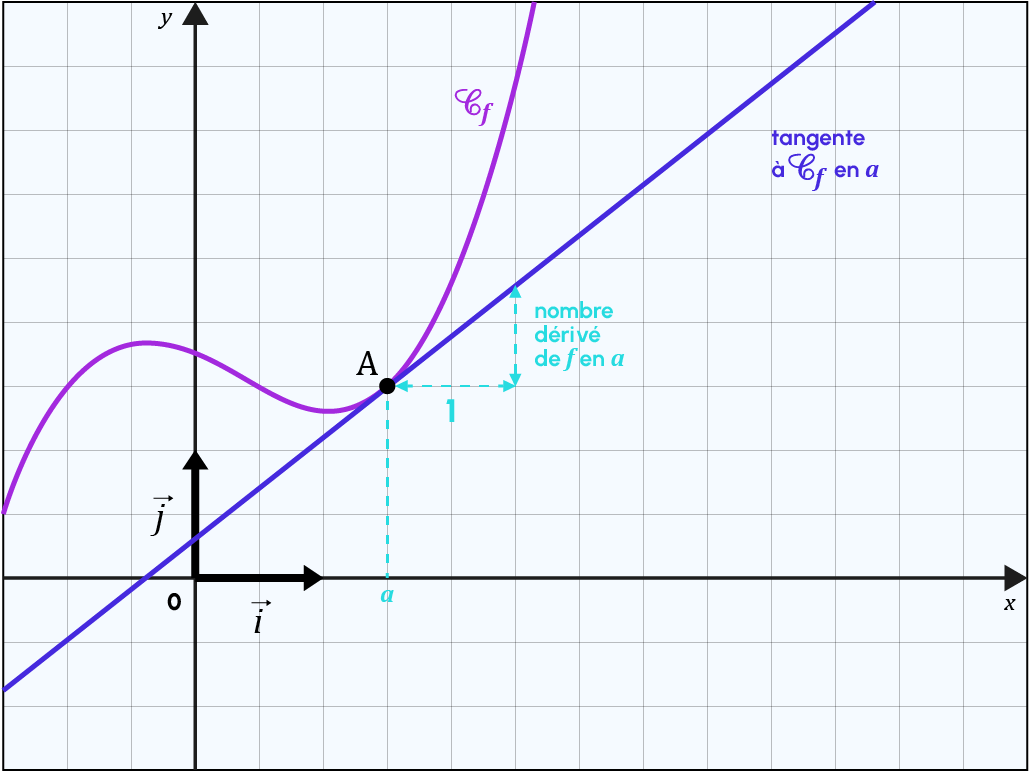
\includegraphics[width=0.5\textwidth]{./images/tangente.png} % Ajustez la largeur
	\caption{Représentation d'une tangente}
	\label{fig:tangente} % Pour référencer l’image
\end{figure}

Le signe de la dérivée permet d’indiquer les variations de la fonction $f$. C’est ce qui représente la tangente à la fonction. Et la dérivée elle-même représente le coefficient directeur de la tangente à $f$ au point. \newline

Une dérivé est représenter par le coefficient directeur de la tangente :
\begin{figure}[h] % h = ici, t = en haut, b = en bas, p = page séparée
	\centering
	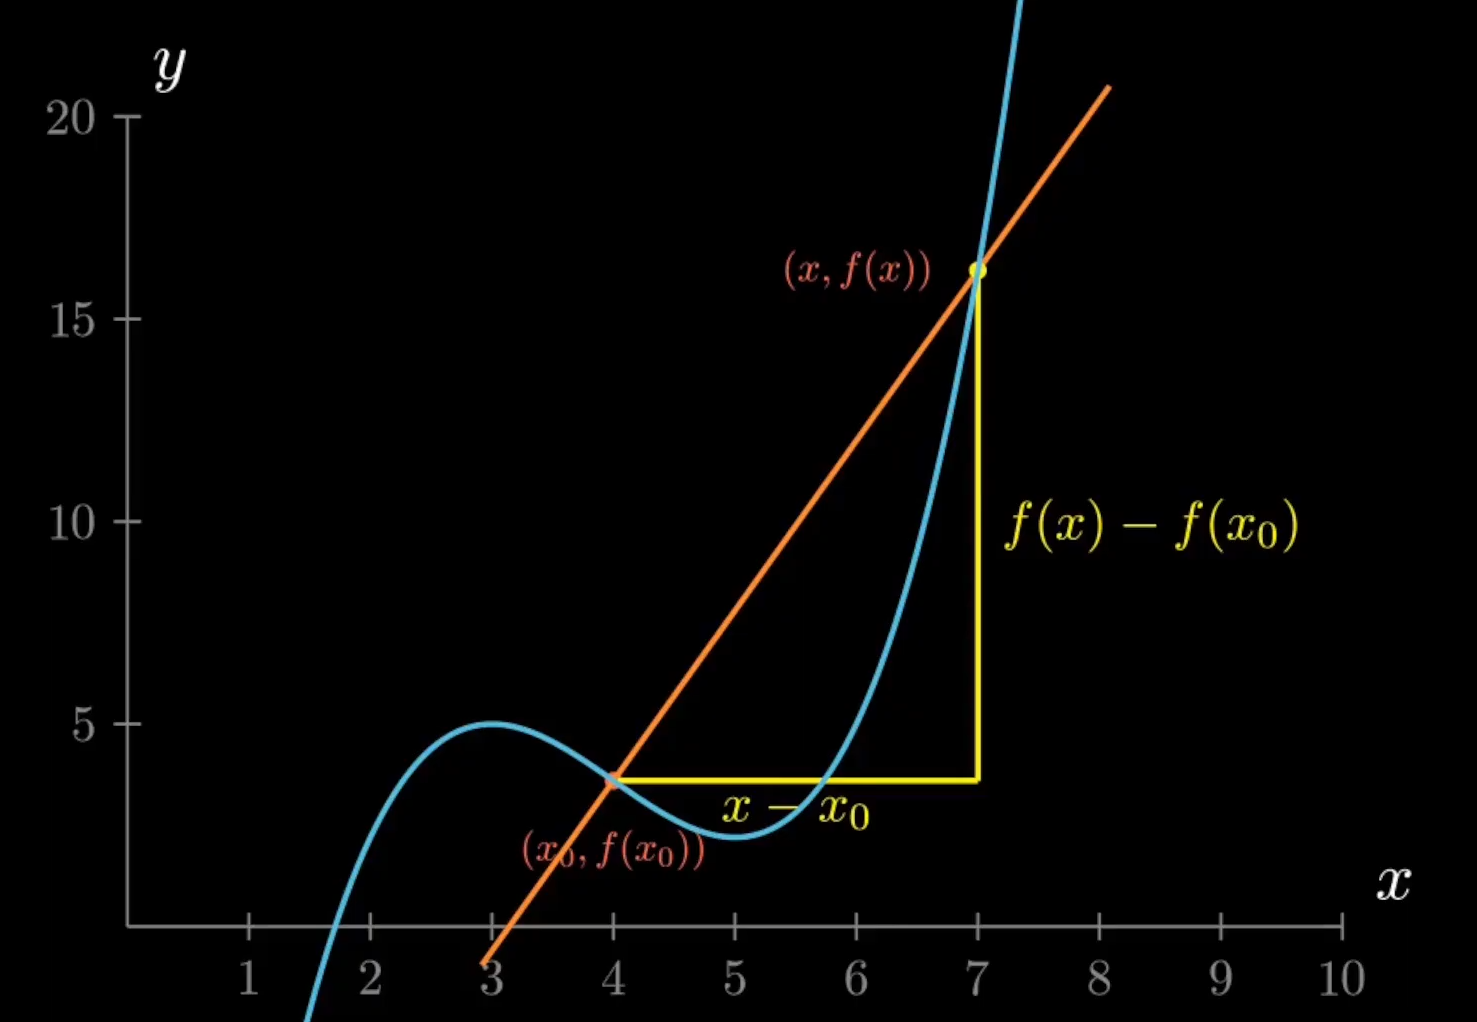
\includegraphics[width=0.5\textwidth]{./images/coef_directeur.png} % Ajustez la largeur
	\caption{Représentation du coefficient directeur}
	\label{fig:coef_directeur} % Pour référencer l’image
\end{figure}

Donc par déduction, c'est la limite de ce coefficient directeur vers le point $(x_{0}, f(x_{0}))$ \newline
Nous avons donc :
\[
\boxed{ f'(x_{0}) = \lim\limits_{x \to x_{0}} \frac{f(x)-f(x_{0})}{x-x_{0}} }
\]
Une fonction peut ne pas avoir de dérivé en tout point de celle-ci.\newline


\begin{figure}[H] % h = ici, t = en haut, b = en bas, p = page séparée
	\centering
	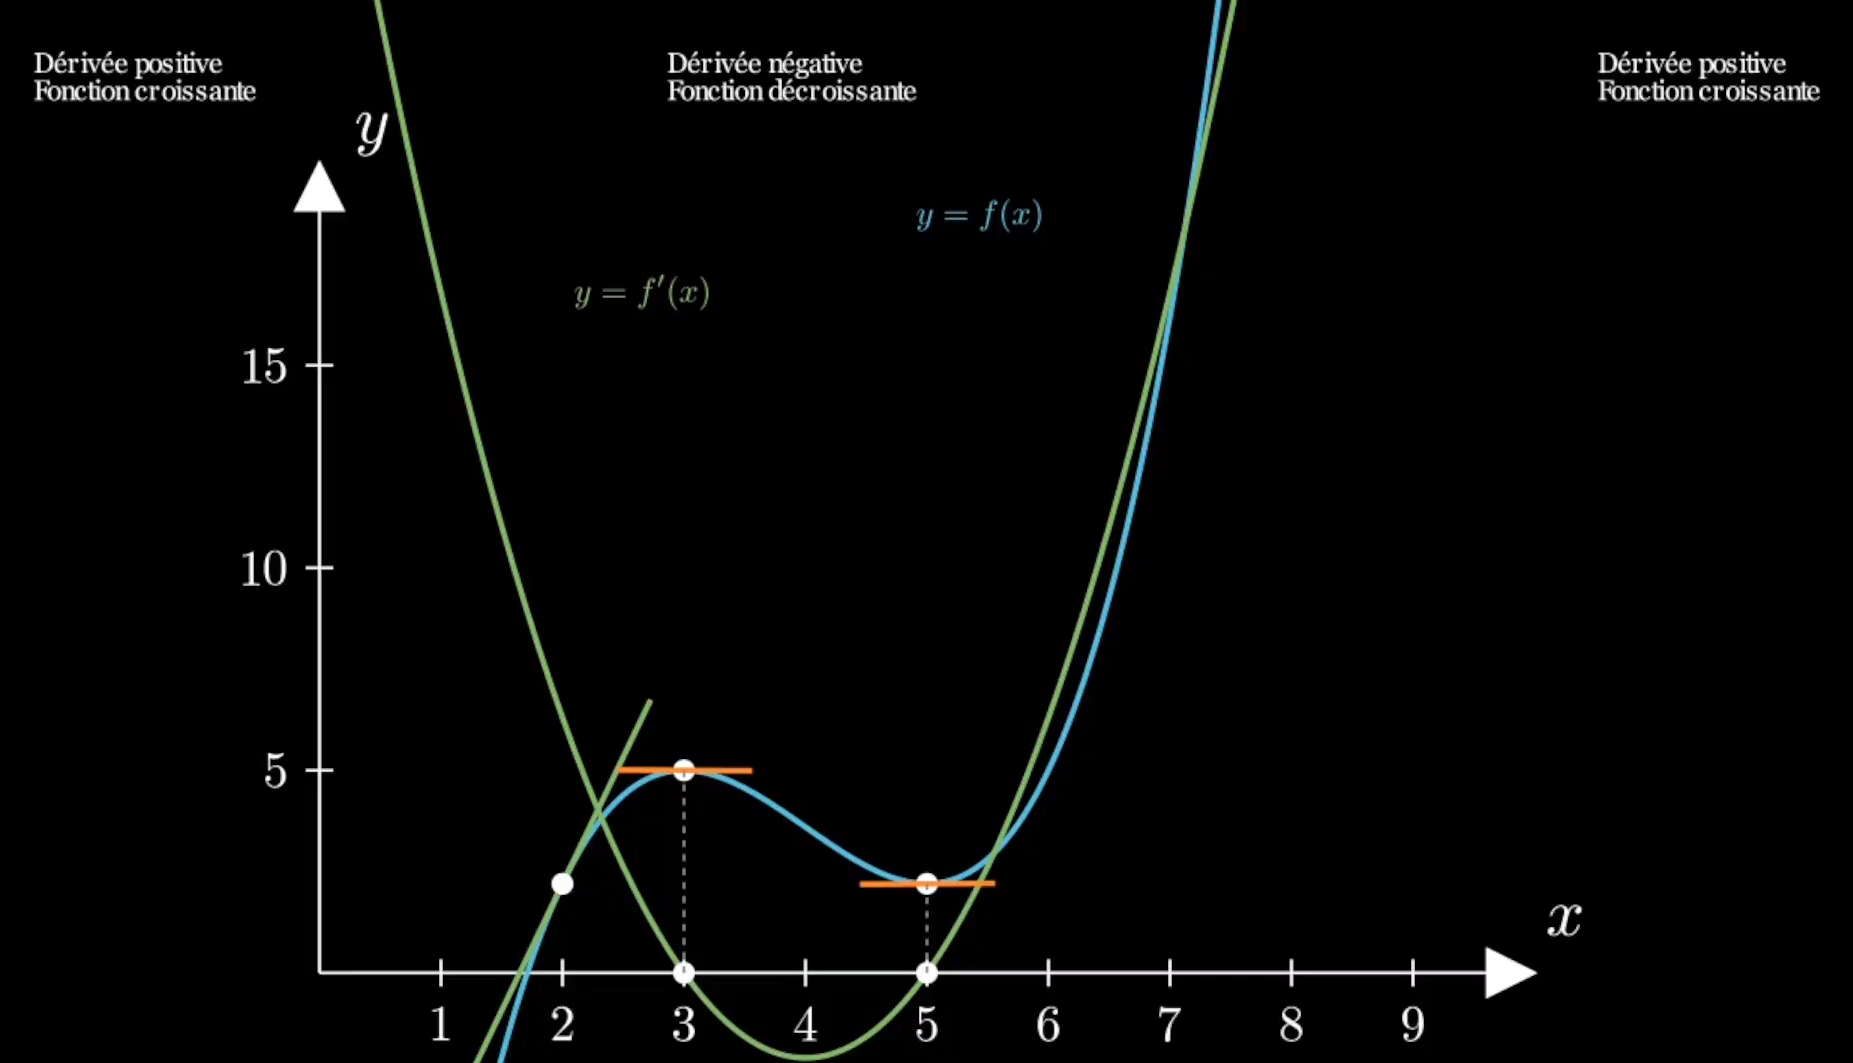
\includegraphics[width=0.5\textwidth]{./images/variations.png} % Ajustez la largeur
	\caption{Déduire le signe de la fonction}
	\label{fig:variations} % Pour référencer l’image
\end{figure}

Grâce à $f'(x)$ nous pouvons voir ici que les points où elle s'annule sont les changements de variation de la fonction $f(x)$.

\newpage
\subsection{Dérivés des fonctions usuelles}
\large
\begin{longtable}{|c|c|c|}
	\caption{Tableau des dérivés usuelles} \label{tab:derives} \\
	
	\hline
	Fonction $f$ & Dérivé $f'$ & Domaine de définition $D_f$ \\
	\hline
	\endfirsthead  % En-tête de la première page
	
	\hline
	Fonction $f$ & Dérivé $f'$ & Domaine de définition $D_f$ \\
	\hline
	\endhead  % En-tête pour les pages suivantes
	
	\hline
	\endfoot  % Pied de page pour chaque page
	
	\hline
	\endlastfoot  % Pied de page pour la dernière page
	
	% Données du tableau
	$f(x) = a$ & $f'(x) = 0$ & $\R$ \\
	$f(x) = x$ & $f'(x) = 1$ & $\R$ \\
	$f(x) = x^n$ & $f'(x) = nx^{n-1}$ & $\R, n \in \N^*$ \\
	$f(x) = \frac{1}{x}$ & $f'(x) = -\frac{1}{x^2}$ & $\left]-\infty, 0\right[ \cup \left]0, +\infty\right[$ \\
	$f(x) = \frac{1}{x^n}$ & $f'(x) = -\frac{n}{x^{n+1}}$ & $\left]-\infty, 0\right[ \cup \left]0, +\infty \right[$ \\
	$f(x) = \sqrt{x}$ & $f'(x) = \frac{1}{2\sqrt{x}}$ & $\R_+$ \\
	$f(x) = ln(x)$ & $f'(x) = \frac{1}{x}$ & $\R^*_+$ \\
	$f(x) = e^x$ & $f'(x) = e^x$ & $\R$ \\
	$f(x) = sin(x)$ & $f'(x) = cos(x)$ & $\R$ \\
	$f(x) = cos(x)$ & $f'(x) = -sin(x)$ & $\R$ \\
	$f(x) = tan(x)$ & $f'(x) = 1 + tan^2(x) = \frac{1}{cos^2(x)}$ & $\R \backslash \left\{\frac{\pi}{2}+k\pi, k \in \Z\right\} $ \\
	
	\hline
	$f(x) = u$ & $f'(x) = u'$ & $$ \\
	$f(x) = u^n$ & $f'(x) = nu'u^{n-1}$ & $$ \\
	$f(x) = \frac{1}{u}$ & $f'(x) = -\frac{u'}{u^2}$ & $$ \\
	$f(x) = \frac{1}{u^n}$ & $f'(x) = -\frac{nu'}{u^{n-1}}$ & $$ \\
	$f(x) = \sqrt{u}$ & $f'(x) = \frac{u'}{2\sqrt{u}}$ & $$ \\
	$f(x) = ln(u)$ & $f'(x) = \frac{u'}{u}$ & $$ \\
	$f(x) = e^u$ & $f'(x) = u'e^u$ & $$ \\
	$f(x) = sin(u)$ & $f'(x) = u'cos(u)$ & $$ \\
	$f(x) = cos(u)$ & $f'(x) = -u'sin(u)$ & $$ \\
	$f(x) = tan(u)$ & $f'(x) = u'(1 + tan^2(u))$ & $$ \\
	$f(x) = u+v$ & $f'(x) = u'+v'$ & $$ \\
	$f(x) = uv$ & $f'(x) = u'v + uv'$ & $$ \\
	$f(x) = \frac{u}{v}$ & $f'(x) = \frac{u'v - uv'}{v^2}$ & $$ \\
	$f(x) = au$ & $f'(x) = au'$ & $$ \\
	
	\hline
	$f(x) = (f \circ g)(x)$ & $f'(x) = g'(x)(f'(x) \circ g(x))$ & $$ \\
\end{longtable}

\newpage
\section{Les primitives usuelles}

\large
\begin{longtable}{|c|c|c|}
	\caption{Tableau des primitives usuelles} \label{tab:primitives} \\
	
	\hline
	Fonction $f$ & Primitives $F$ & Domaine de définition $D_f$ \\
	\hline
	\endfirsthead  % En-tête de la première page
	
	\hline
	Fonction $f$ & Primitives $F$ & Domaine de définition $D_f$ \\
	\hline
	\endhead  % En-tête pour les pages suivantes
	
	\hline
	\endfoot  % Pied de page pour chaque page
	
	\hline
	\endlastfoot  % Pied de page pour la dernière page
	
	% Données du tableau
	$f(x) = k$ & $F(x) = kx+C$ & $\R$ \\
	$f(x) = x$ & $F(x) = \frac{x^2}{2}$ & $\R$ \\
	$f(x) = x^n$ & $F(x) = \frac{x^{n+1}}{n+1}+C$ & $n \in \Z \backslash \left \{-1;0 \right \}$ \\
	$f(x) =a^x$ & $F(x) = \frac{a^{x}}{ln(a)}+C$ & $\R$ \\
	$f(x) = \frac{1}{x}$ & $F(x) = ln(|x|)+C$ & $\R^{*}$ \\
	$f(x) = \frac{1}{x^n}$ & $F(x) = -\frac{1}{(n-1)x^{n-1}}+C$ & $\left]-\infty, 0\right[ \cup \left]0, +\infty \right[$ \\
	$f(x) = \frac{1}{\sqrt{x}}$ & $F(x) = 2\sqrt{x}+C$ & $\R_+$ \\
	$f(x) = ln(x)$ & $F(x) = xln(x)-x+C$ & $\R^*_+$ \\
	$f(x) = e^x$ & $F(x) = e^x+C$ & $\R^*_+$ \\
	$f(x) = sin(x)$ & $F(x) = -cos(x)+C$ & $\R$ \\
	$f(x) = cos(x)$ & $F(x) = sin(x)+C$ & $\R$ \\
	$f(x) = tan(x)(x)$ & $F(x) = -ln(|cos(x)|)+C$ & $\R - \left\{ \frac{\pi}{2} + k\pi \right\}$ \\
	$f(x) = 1+tan^2(x) = \frac{1}{cos^2(x)}$ & $F(x) = tan(x)+C$ & $ \left]-\frac{\pi}{2}+k\pi, \frac{\pi}{2}+k\pi \right[, k \in \Z$ \\
	
	\hline
	$f(x) = u'u^n$ & $F(x) = \frac{u^{n+1}}{n+1}+C$ & $n \in \Z \backslash \left \{-1;0 \right \}$ \\  
	$f(x) = \frac{u'}{\sqrt{u}}$ & $F(x) = 2\sqrt{u}+C$ & $\R$ \\  
	$f(x) = \frac{u'}{u^2}$ & $F(x) = -\frac{1}{u}+C$ & $n \in \N, n \geq 2$ \\  
	$f(x) = \frac{u'}{u^n}$ & $F(x) = -\frac{1}{(n-1)u^{n-1}}+C$ & $n \in \N, n \geq 2$ \\  
	$f(x) = \frac{u'}{u}$ & $F(x) = ln(|u|)+C$ & $\R$ \\  
	$f(x) = u'e^{u}$ & $F(x) = e^{u}+C$ & $\R$ \\  
	$f(x) = u'cos(u)$ & $F(x) = sin(u)+C$ & $\R$ \\  
	$f(x) = u'sin(u)$ & $F(x) = -cos(u)+C$ & $\R$ \\  
	$f(x) = u'tan(u)$ & $F(x) = -ln | cos(u) | + C$ & $\R - \left\{ \frac{\pi}{2} + k\pi \right\}$ \\  
	
\end{longtable}


\end{document}